\documentclass[a4paper,12pt]{article}
\usepackage{graphicx}

\title{InsituNet Application for Cytoscape \\ \large User Documentation}

\begin{document}
\maketitle
\begin{abstract}
In situ sequencing is a novel method to generate spatially-resolved, in situ RNA localization and expression data, at an almost single-cell resolution. Few methods, however, currently exist to analyze and visualize the complex data produced, which can encode the localization and expression of a million or more individual transcripts in a tissue section. Here, we present InsituNet, an innovative new application that converts in situ sequencing data into interactive network-based visualizations, where each unique transcript is a node in the network and edges represent the spatial co-expression relationships between transcripts. InsituNet enables the analysis of the relationships that exist between these transcripts and can uncover how spatial co-expression profiles change in different regions of the tissue or across different tissue sections. 
\end{abstract}
\clearpage

\tableofcontents

\clearpage

\section{Introduction}
Welcome to the InsituNet user documentation. This documentation aims to be a complete description of the functionality and user-interface of InsituNet. It also contains step-by-step examples of using InsituNet to analyze and visualize spatially-aware gene expression data.

\begin{figure}[htb]
	\caption{Screenshot of Cytoscape 3.5.1 running InsituNet}\label{fig:shot}
	\centering
	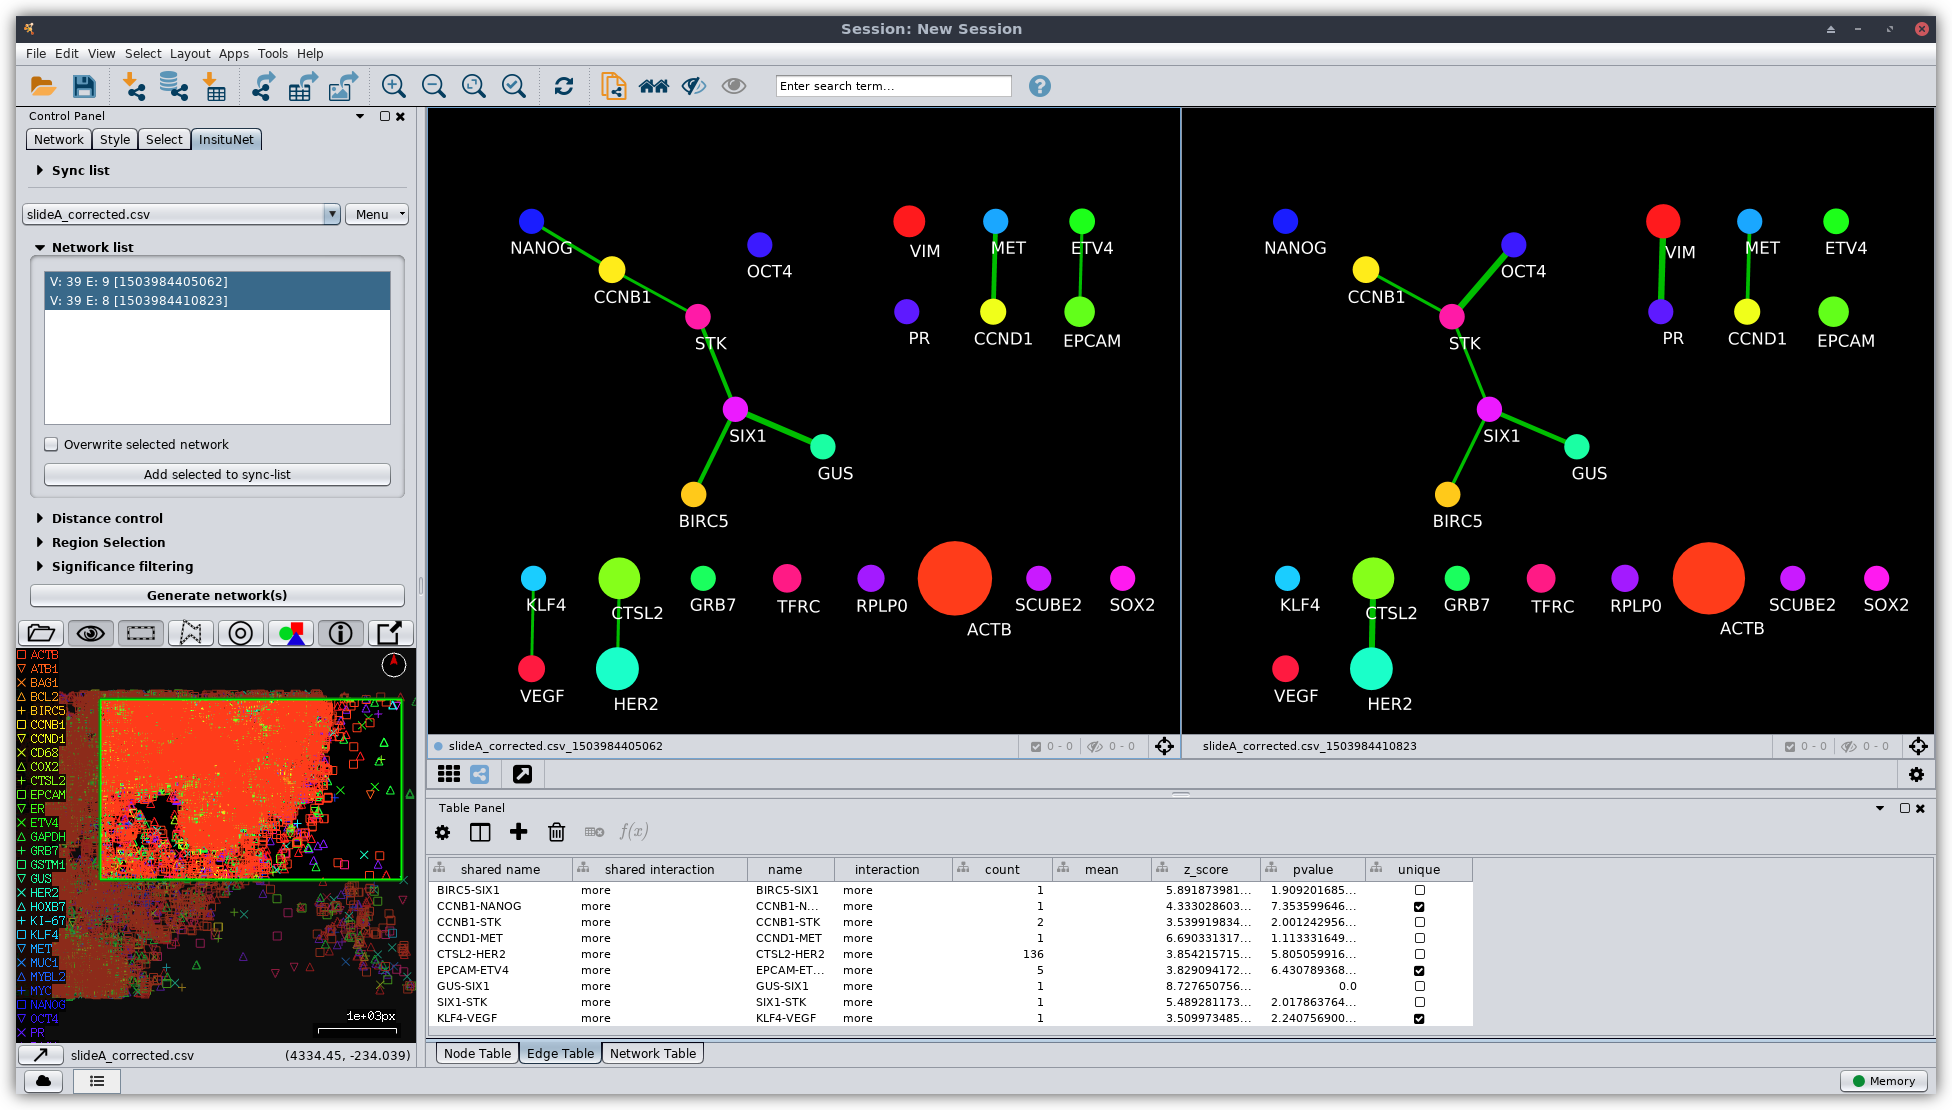
\includegraphics[width=\textwidth]{shot_1-shadow}
\end{figure}

\subsection{Overview}
InsituNet is an app (plugin) that runs inside of Cytoscape. Its chief purpose is taking \emph{in situ} sequencing data and allowing it to be visually explored and profiled such as in Figure \ref{fig:recon}, and creating co-expression networks from it such as the one in Figure \ref{fig:shot}.
\begin{figure}[h]
	\caption{InsituNet's reconstruction of the \emph{in situ} sequencing data.}\label{fig:recon}
	\centering
	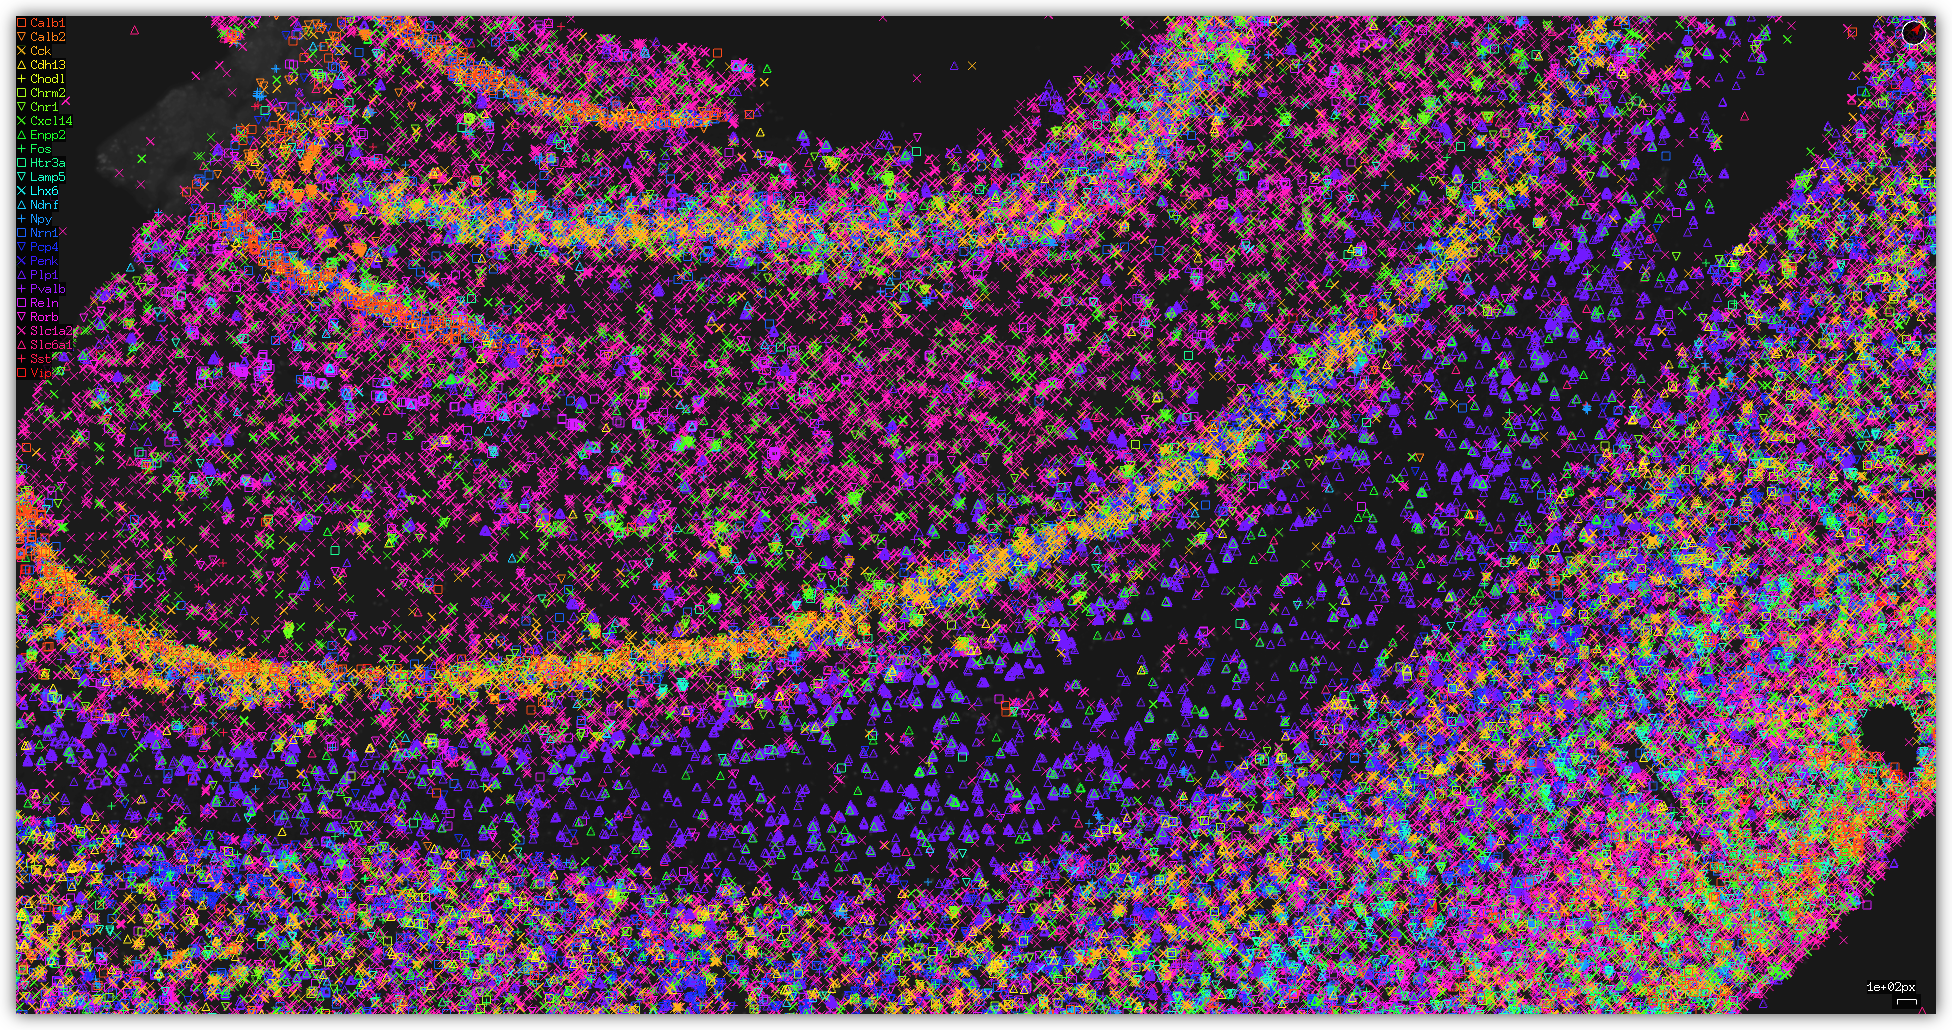
\includegraphics[width=\textwidth]{reconstruction-shadow}
\end{figure}

The networks represent \emph{spatial co-expression} relationships. If you have two nodes joined by a link you know that the two transcripts those nodes represent are close by each other (at least once). InsituNet also provides options for filtering these relationships so that only the most significant co-expressions are shown as edges. The distance used as "co-expression distance" is also user-adjustable, and you may wish to make it longer or shorter depending on whether you are interested in inter or intra-cellular distances.

\subsection{Input format}
InsituNet requires a file of comma-separated values (csv) as input. In this file, there should be at least 3 columns, one for the name of the transcript, and two for x and y coordinates. The first row in the csv file should be headers (eg. name, x, y). Each row after the header represents a single transcript detection. The exact name of the headers and their order is not important as you will be prompted to check that the correct columns are selected on import. An example input file is seen here:

\begin{center}
\begin{tabular}{ l c r }
	\centering
	name & xpos & ypos \\ \hline
	ACTB & 5.04 & 6.35 \\
	GAPDH & 9.66 & 4.13 \\
	ACTB & 7.65 & 2.21 \\
\end{tabular}
\end{center}

\section{InsituNet control panel}

The InsituNet control panel is the central point for managing all aspects of InsituNet. It contains various collapsible sub-panels, each controlling a different aspect of how networks are created. This panel is only visible once a dataset has been successfully imported. On successful import, the name of the file will be visible at the top of the panel, in a combobox. This box allows switching between different datasets in the case that you import more than one. Directly to the right is a menubutton containing options for the selected dataset. `About' will allow the user to see how many unique types, and how many transcripts in total are within the selected dataset. `Delete' is reasonable self-explanatory. Directly below this is the sync-subpanel. This is initially empty, but when you choose to synchronise the layouts of your networks, those networks will appear here. You can also choose which layout algorithm to use, and remove datasets as required. An additional option is available to highlight unique edges, which will change the network style to display edges that only occur in one synchronised dataset in red.

\subsection{Network list}
All the controls mentioned so far have been global; that is, they are not dataset-specific. All controls from here on will be applied specifically to the currently selected dataset. The first of the dataset-specific subpanels is the Network List. The network list panel contains all networks generated for this dataset. When clicked, the current network view will switch the the selected network. This panel also contains the `Overwrite selected network' option, which causes whatever network is highlighted to be reused when you generate a network (the default behaviour is to create a new entry)\footnote{Tip: If you are simply exploring a dataset or testing the parameters and don't need to retain the networks you are generating, it is recommended to use this option, as it will prevent your network list from becoming needlessly cluttered. Make sure to turn it off again if you generate a network you want to keep!}, as well as synchronisation-specific options.

\subsection{Distance control}
In the distance control panel the pixel distance to be used for defining co-expression may be set. This is also converted into microns at the given magnification for convenience.
\subsection{Region selection}
The region selection panel provides the option to use an automatic sliding window of given dimensions. If this is chosen, the dataset will be divided into the chosen number of rectangular windows with the given overlap. This panel also provides the option for using the full dataset as background. This changes the co-expression significance calculations to take into account the total abundance, rather than just the abundance within the selection area.
\subsection{Significance filtering}
The main panel for adjusting how significance is assessed. There are three test options, Label shuffle, hypergeometric test, and no filtering. No filtering will cause any co-expressed transcripts to have an edge drawn between them. The label shuffle and hypergeometric tests will both attempt to rate the significance of edges, as described in more detail in the next section.


\subsection{Tissue reconstruction}
The tissue reconstruction is likely where you will start in order to explore and check the data that you have just imported. It can initially be found at the bottom of the InsituNet panel. This view can be panned (left click + drag), zoomed (mouse wheel), and rotated (wheel / middle button + drag vertically) using the mouse. The controls as numbered in \ref{fig:recon_details} are as follows:

\begin{enumerate}
	\item Open menu: This can be used to import imagery that will be displayed behind the transcripts.
	\item Toggle show all: A toggle button that switches between showing all transcripts, or showing only those transcripts that correspond to the current selection within the network.
	\item Rectangular selection mode: When this is enabled, right clicking + dragging will draw a rectangle from which the network will be generated.
	\item Polygonal selection mode: In this mode, right clicking will place a polygon point, clicking + dragging will draw a continuous line. Any polygonal shape may be drawn, but the end must meet the beginning!
	\item Reset view: Will center and scale the view to fit within the current window size.
	\item Appearance editor: Pops up a window that allows transcript colours, symbols, and sizes to be customised.
	\item Toggle info: Will toggle the visibility of legend and other non-transcript information.
	\item Export: Provides options for exporting the current tissue reconstruction view as an image.
	\item Legend: Lists transcript names, colours and symbols.
	\item Compass: Points "North" (the positive Y direction).
	\item Scalebar: Shows current scale in pixel distance.
	\item Infobar: Provides some information such as dataset name, cursor coordinates, and the pin/unpin button for floating the window.
\end{enumerate}


\begin{figure}[htb]
	\caption{The tissue reconstruction window, and accompanying toolbar.}\label{fig:recon_details}
	\centering
	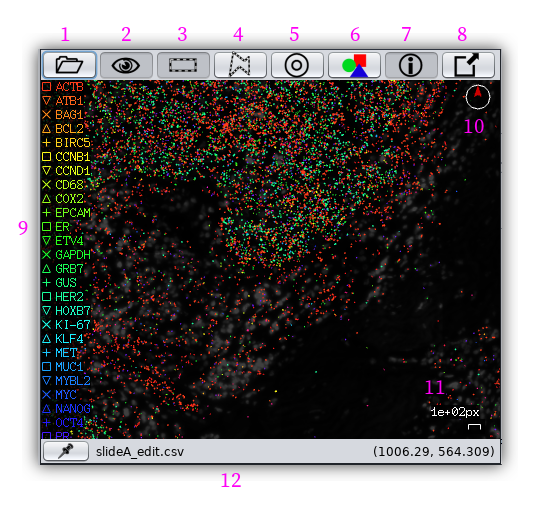
\includegraphics[width=\textwidth]{recon_details-shadow}
\end{figure}

\section{Network generation in detail}
There are essentially two steps to generating InsituNet's networks: Firstly the number of co-expressions between all transcript pairs must be found, and secondly a significance attached assessed for these pairs.

\subsection{Finding co-expressions}
On import of a dataset, InsituNet creates a space-partitioning kd-tree in order to be able to rapidly find neighbours and perform various other range queries. This datastructure is then queried when a new network is generated to find all transcripts within a set euclidean distance of each other, as defined in the distance control panel.

\subsection{Edge filtering}
\subsection{Filtering (shuffle)}
With a real dataset, this network will need aditional filtering to be useful, as there will likely be issues with edge density. InsituNet provides various options for filtering the networks as they are created. The simplest filtering option is no filtering. This will create a network in which an edge is drawn between transcripts that exhibit any co-expression at all. No assessment of significance is made. The other options are the shuffle and hypergeometric methods, are both statistical methods for pruning edges in order to display only those interactions that are significant given the context.
In situ sequencing provides extremely dense data on the detection of 1 million or more transcripts in a given tissue section. In such dense data, we would expect to observe a large number of co-expressions simply by chance, particularly for highly abundant transcripts. InsituNet aims to identify co-expressions between two transcripts that occur statistically more than expected given the abundance of the two transcripts in the data. These statistically significant interactions are more likely to represent true functional co-expressions. InsituNet can also identify transcripts that are co-expressed much less than expected given their abundance, as these transcripts may represent specific biomarkers of particular cell-types or tissue regions (e.g. those associated with pathology).
\subsection{Filtering (hypergeometric)}

\section{Miscellaneous}

\end{document}
